%%%%%%%%%%%%%%%%%%%%%%%%%%%%%%%%%%%%%%%%%
% Beamer Presentation
% LaTeX Template
% Version 1.0 (10/11/12)
%
% This template has been downloaded from:
% http://www.LaTeXTemplates.com
%
% License:
% CC BY-NC-SA 3.0 (http://creativecommons.org/licenses/by-nc-sa/3.0/)
%
%%%%%%%%%%%%%%%%%%%%%%%%%%%%%%%%%%%%%%%%%

%----------------------------------------------------------------------------------------
%   PACKAGES AND THEMES
%----------------------------------------------------------------------------------------

\documentclass{beamer}

\mode<presentation> {

% The Beamer class comes with a number of default slide themes
% which change the colors and layouts of slides. Below this is a list
% of all the themes, uncomment each in turn to see what they look like.

%\usetheme{default}
%\usetheme{AnnArbor}
%\usetheme{Antibes}
%\usetheme{Bergen}
%\usetheme{Berkeley}
%\usetheme{Berlin}
%\usetheme{Boadilla}
%\usetheme{CambridgeUS}
%\usetheme{Copenhagen}
%\usetheme{Darmstadt}
%\usetheme{Dresden}
%\usetheme{Frankfurt}
%\usetheme{Goettingen}
%\usetheme{Hannover}
%\usetheme{Ilmenau}
%\usetheme{JuanLesPins}
%\usetheme{Luebeck}
\usetheme{Madrid}
%\usetheme{Malmoe}
%\usetheme{Marburg}
%\usetheme{Montpellier}
%\usetheme{PaloAlto}
%\usetheme{Pittsburgh}
%\usetheme{Rochester}
%\usetheme{Singapore}
%\usetheme{Szeged}
%\usetheme{Warsaw}

% As well as themes, the Beamer class has a number of color themes
% for any slide theme. Uncomment each of these in turn to see how it
% changes the colors of your current slide theme.

%\usecolortheme{albatross}
%\usecolortheme{beaver}
%\usecolortheme{beetle}
%\usecolortheme{crane}
%\usecolortheme{dolphin}
%\usecolortheme{dove}
%\usecolortheme{fly}
%\usecolortheme{lily}
%\usecolortheme{orchid}
%\usecolortheme{rose}
%\usecolortheme{seagull}
%\usecolortheme{seahorse}
%\usecolortheme{whale}
%\usecolortheme{wolverine}

%\setbeamertemplate{footline} % To remove the footer line in all slides uncomment this line
%\setbeamertemplate{footline}[page number] % To replace the footer line in all slides with a simple slide count uncomment this line

%\setbeamertemplate{navigation symbols}{} % To remove the navigation symbols from the bottom of all slides uncomment this line
}

\usepackage{graphicx} % Allows including images
\usepackage{booktabs} % Allows the use of \toprule, \midrule and \bottomrule in tables

\usepackage{tikz}
\def\checkmark{\tikz\fill[scale=0.4](0,.35) -- (.25,0) -- (1,.7) -- (.25,.15) -- cycle;} 

\usepackage{fourier}

% Locale
\usepackage[portuguese]{babel}
\uselanguage{Portuguese}
\languagepath{Portuguese}

%----------------------------------------------------------------------------------------
%   TITLE PAGE
%----------------------------------------------------------------------------------------

\title[Algoritmos Gulosos]{Material Didático sobre Algoritmos Gulosos} % The short title appears at the bottom of every slide, the full title is only on the title page

\author{Victor de Oliveira Colombo} % Your name
\institute[IME-USP] % Your institution as it will appear on the bottom of every slide, may be shorthand to save space
{
Instituto de Matemática e Estatística da Universidade de São Paulo \\ % Your institution for the title page
\medskip
\textit{victor.colombo@usp.br} % Your email address
}
\date{26 de Novembro de 2018} % Date, can be changed to a custom date

\begin{document}

\begin{frame}
\titlepage % Print the title page as the first slide
\end{frame}

% \begin{frame}
% \frametitle{Overview} % Table of contents slide, comment this block out to remove it
% \tableofcontents % Throughout your presentation, if you choose to use \section{} and \subsection{} commands, these will automatically be printed on this slide as an overview of your presentation
% \end{frame}

%----------------------------------------------------------------------------------------
%   PRESENTATION SLIDES
%----------------------------------------------------------------------------------------

%------------------------------------------------
\section{First Section} % Sections can be created in order to organize your presentation into discrete blocks, all sections and subsections are automatically printed in the table of contents as an overview of the talk
%------------------------------------------------

\subsection{Subsection Example} % A subsection can be created just before a set of slides with a common theme to further break down your presentation into chunks

\begin{frame}
\frametitle{Objetivos}
\begin{itemize}

\item Resolver problemas que utilizem algoritmos gulosos aliados a outros tópicos.

\item Desenvolver o raciocínio e a intuição por trás das técnicas gulosas

\item Criar uma ferramenta sistemática para resolver problemas dessa classe.

\item Apresentar algoritmos gulosos de uma maneira pragmática, a partir de problemas
de competições de programação.

\item Destoar dos problemas clássicos que são frequentemente abordados nos livros-texto.
\end{itemize}
\end{frame}

%------------------------------------------------

\begin{frame}
\frametitle{Problema da Mochila}
\begin{itemize}
\item São dados $n$ itens e uma mochila de tamanho $S$.

\item Cada item tem um peso $w_i$ e um valor $v_i$.

\item Escolher subconjunto  de itens $I \subseteq [1, n]$ tal que $$\sum_{i \in I}w_i \leq S$$

\item Maximizar $$\sum_{i \in I}v_i$$
\end{itemize}
\end{frame}

%------------------------------------------------

\begin{frame}
\frametitle{Problema da Mochila - Programação Dinâmica}

\begin{itemize}
\item Seja $f(i, s)$ o valor máximo para o subproblema considerando os itens $i, i + 1, ..., n$ e uma mochila de tamanho $s$.
\end{itemize}
 
\begin{equation}
  f(i, s) =
  \begin{cases}
  0                                                             & \text{se $i = n + 1$} \\
  max(f(i + 1, s), v_i + f(i + 1, s - w_i))   & \text{se $w_i \leq s$} \\
  f(i + 1, s)                                          & \text{c.c.} \\
  \end{cases}
\end{equation}

\begin{itemize}
\item Resposta é $f(1, S)$
\item Programação Dinâmica: complexidade de tempo $O(nS)$
\end{itemize}

\end{frame}

%------------------------------------------------

\begin{frame}
\frametitle{Problema da Mochila modificado}
\begin{itemize}
\item São dados $n$ itens e uma mochila de tamanho $S$.

\item Cada item tem um peso $w_i$ \textbf{após} de ser colocado na mochila, um peso $c_i$ \textbf{antes} de ser colocado na mochila e um valor $v_i$.

\item Para todo item, $c_i \geq w_i$.

\item Escolher subconjunto  de itens $I \subseteq [1, n]$ e uma permutação $r$ de $I$ tal que, para todo $j$, $$c_{r_j} + \sum_{i = 1}^{j - 1} w_{r_i} \leq S$$

\item Maximizar $$V(I) = \sum_{i \in I}v_i$$
\end{itemize}
\end{frame}

%------------------------------------------------

\begin{frame}
\frametitle{Problema da Mochila modificado - Exemplo 1}
\begin{itemize}
\item $S = 5$, $n = 4$, $v = \{1, 2, 3, 1\}$, $c = \{3, 2, 3, 4\}$, $w = \{1, 2, 2, 4\}$
\item A escolha $I = \{1, 2, 3\}$ e $r = \{1, 2, 3\}$ não é válida, já que:
    \begin{itemize}
      \item $c_1 = 3 < S$ \checkmark
      \item $c_2 + w_1 = 2 + 1 = 3 < S$ \checkmark
      \item $c_3 + w_2 + w_1 = 3 + 2 + 1 = 6 > S$ \danger
    \end{itemize}
\end{itemize}
\end{frame}

%------------------------------------------------

\begin{frame}
\frametitle{Problema da Mochila modificado - Exemplo 2}
\begin{itemize}
\item $S = 5$, $n = 4$, $v = \{1, 2, 3, 1\}$, $c = \{3, 2, 3, 4\}$, $w = \{1, 2, 2, 4\}$
\item A escolha $I = \{1, 2, 3\}$ e $r = \{3, 1, 2\}$ é válida e ótima, já que:
    \begin{itemize}
      \item $c_3 = 3 < S$ \checkmark
      \item $c_1 + w_3 = 3 + 2 = 5 = S$ \checkmark
      \item $c_2 + w_1 + w_3 = 2 + 1 + 2 = 5 = S$ \checkmark
      \item $V(I) = 6$ é máximo
    \end{itemize}
\end{itemize}
\end{frame}

%------------------------------------------------

\begin{frame}
\frametitle{Problema da Mochila modificado - Programação Dinâmica?}

\begin{equation}
  f'(i, s) =
  \begin{cases}
  0                                                             & \text{se $i = n + 1$} \\
  max(f'(i + 1, s), v_i + f'(i + 1, s - w_i))   & \text{se $\boldsymbol{c_i \leq s}$} \\
  f'(i + 1, s)                                          & \text{c.c.} \\
  \end{cases}
\end{equation}

\begin{itemize}
\item A recorrência assume ordem fixa!
\item Escolhe elementos de maneira sequencial...
\item Aplicar recorrência para toda permutação de itens? Podemos fazer melhor!
\end{itemize}

\end{frame}

%------------------------------------------------

\begin{frame}
\frametitle{Ordenação gulosa}

\begin{itemize}
\item Podemos ``desconfiar'' de uma ordenação gulosa.
\item Ideia 1: Inserir elementos em ordem decrescente de $c$
    \begin{itemize}
    \item Falso!
    \end{itemize}
\item Ideia 2: Inserir elementos em ordem decrescente de $c - w$
    \begin{itemize}
    \item Verdadeiro?
    \end{itemize}
\end{itemize}

\end{frame}

%------------------------------------------------

\begin{frame}
\frametitle{Formalização}
\frametitle{Teorema}
\begin{theorem}
Se $I \subseteq [1, n]$ é um subconjunto ótimo de itens e $r$ é uma permutação de $I$ tal que $c_{r_i} - w_{r_i} \geq c_{r_j} - w_{r_j}$ para todo $i \leq j$, então $r$ é uma permutação válida.
\end{theorem}
Definiremos uma função $F(p)$ para uma permutação $p$ como o número de pares de índices $(i, j)$, $i \leq j$, tal que $c_{p_i} - w_{p_i} < c_{p_j} - w_{p_j}$.\\~\\

Por construção, $F(r) = 0$. \\~\\

Suponha que $r$ não seja uma permutação válida.

\end{frame}

%------------------------------------------------

\begin{frame}
\frametitle{Demonstração}


Seja $r^*$ uma permutação válida de $I$ com menor valor de $F(r^*) > 0$. Seja $t \in [1, |I| - 1]$ o primeiro índice tal que $c_{r^*_t} - w_{r^*_t} < c_{r^*_{t + 1}} - w_{r^*_{t + 1}}$.\\~\\

Seja $S^* = S - \sum_{i = 1}^{t - 1} w_{r^*_i}$. Para $r^*$ ser uma permutação válida, temos as condições:

$$c_{r^*_t} \leq S^*$$
$$c_{r^*_{t + 1}} \leq S^* - w_{r^*_t}$$

\end{frame}

%------------------------------------------------

\begin{frame}
\frametitle{Demonstração - cont.}

\begin{itemize}
\item Ora mas como $t$ é uma ``inversão'', vale que:

$$c_{r^*_t} - w_{r^*_t} < c_{r^*_{t + 1}} - w_{r^*_{t + 1}}$$

\item Juntando com as equaçãoes anteriores, temos:

$$c_{r^*_{t}} + w_{r^*_{t + 1}} < c_{r^*_{t + 1}} + w_{r^*_t} \leq S^*$$

\item A sequência $\widetilde{r} = \{r_1, ..., r_{t - 1}, r_t, r^*_{t + 1}, r^*_{t + 2}, ..., r^*_k\}$ é válida e remove pelo menos um par de índices que viola a ordenação gulosa. Assim, temos que $F(\widetilde{r}) < F(r^*)$, uma contradição na hipótese que $F(r^*)$ é mínimo.
\end{itemize}

\end{frame}

%------------------------------------------------

\begin{frame}
\frametitle{Algortimo}

\begin{itemize}
\item Para todo subconjunto ótimo, podemos reordená-lo de acordo com o critério guloso.
\item Agora podemos ordenar para remover a restrição da ordem e aplicar a recorrência $f'(i, s)$ para escolher o subconjunto.
\end{itemize}

\end{frame}

%------------------------------------------------

\begin{frame}
\frametitle{Pseudocodigo}

\begin{figure}
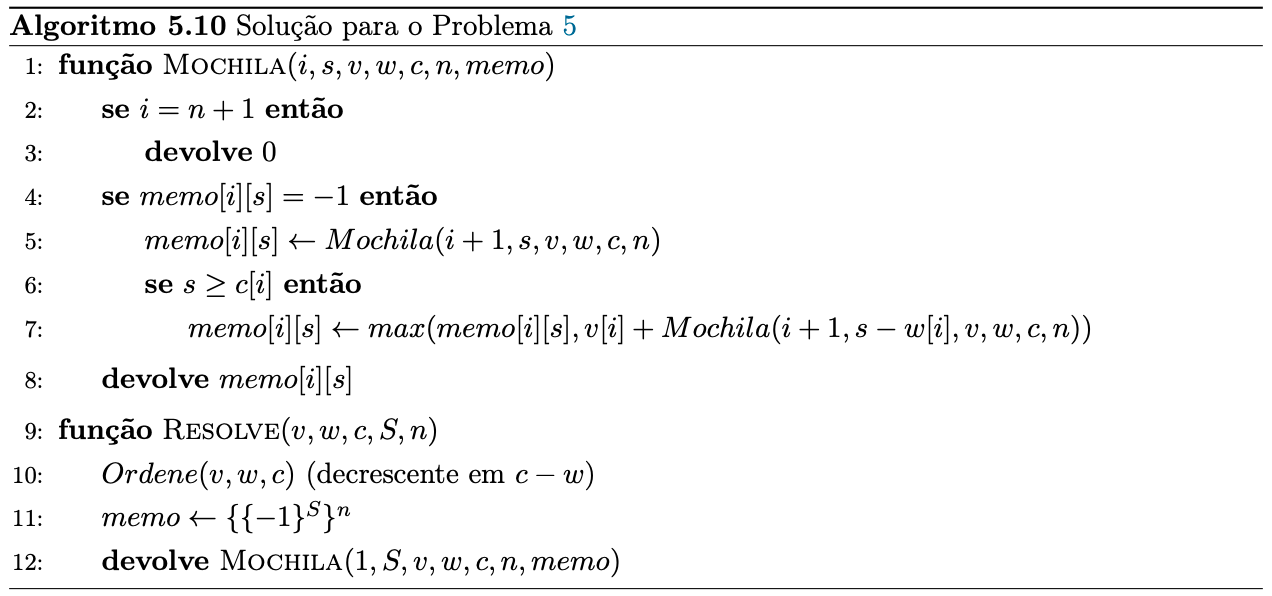
\includegraphics[width=0.8\linewidth]{pseudo.png}
\end{figure}
\begin{itemize}
  \item Complexidade de tempo $O(nS + n \lg n)$ e espaço $O(nS)$.
  \item Possível reduzir o espaço para $O(S)$ numa implementação iterativa. 
\end{itemize}

\end{frame}

%------------------------------------------------

\begin{frame}

\begin{itemize}
\item Perguntas?\\~\\
\item Mais informações em:
\url{https://linux.ime.usp.br/~colombo/mac0499/}
\end{itemize}

\end{frame}

%----------------------------------------------------------------------------------------

\end{document}